\newsection{Installazione}
\subsection{Installazione di Grafana}
Per poter installare e utilizzare il plug-in è necessario scaricare e configurare precedentemente Grafana; le istruzioni di installazione sono reperibili al link\\[0.2cm]
\hspace*{10mm}\url{http://docs.grafana.org/installation/} \\[0.2cm]
che le riassume per ogni sistema operativo supportato.\\
Il plug-in è stato sviluppato utilizzando la versione 5.4.3. Per evitare errori nell'esecuzione, si raccomanda di avvalersi della stessa versione.
Una volta terminata la configurazione descritta al riferimento precedente, in Windows avviare l'eseguibile\\[0.2cm]
\hspace*{10mm}\begin{ttfamily}grafana-5.4.3/bin/grafana-server.exe\end{ttfamily}\\[0.2cm] mentre in Linux eseguire il comando\\[0.2cm]
\hspace*{10mm}\begin{ttfamily}sudo service grafana-server start\end{ttfamily}\\[0.2cm]
A questo punto, aprire una finestra del browser e navigare all'indirizzo URL \url{localhost:3000}. La porta 3000 è quella di default per Grafana, ma su sistema operativo Windows potrebbe richiedere permessi aggiuntivi.
\subsection{Installazione Node.js}
Per usufruire delle funzionalità del plug-in è necessario installare il \gl{framework} Node.js e il relativo gestore dei pacchetti chiamato Node Package Manager (\gl{NPM}), attraverso l'apposita sezione al link\\[0.2cm]
\hspace*{10mm}\url{https://nodejs.org/it/download/}.\\[0.2cm] In questo modo saranno disponibili i comandi \begin{ttfamily}npm install\end{ttfamily} e \begin{ttfamily}npm run build\end{ttfamily}, necessari rispettivamente per l'installazione di tutte le dipendenze specificate nel \gl{package.json} e per l'esecuzione del processo di \gl{build}.
\begin{figure} [H]
	\centerline{
		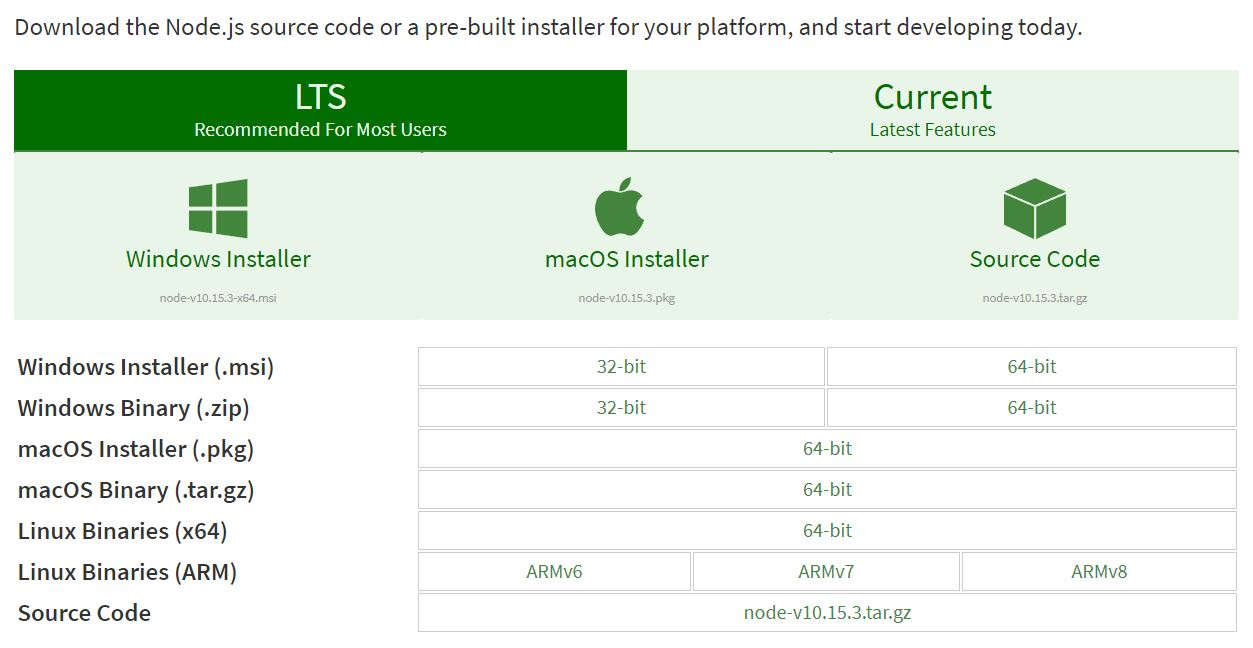
\includegraphics[scale=0.5]{Img/node1}}
	\caption{Pagina di download di Node.js}\label{}
\end{figure}
Verificare, alla fine, la disponibilità del comando \begin{ttfamily}npm\end{ttfamily} tramite il comando \begin{ttfamily}npm -v\end{ttfamily}. In caso negativo, scaricarlo dal link \\[0.2cm]
\hspace*{10mm}\url{https://www.npmjs.com/get-npm/}.
\begin{figure} [H]
	\centerline{
		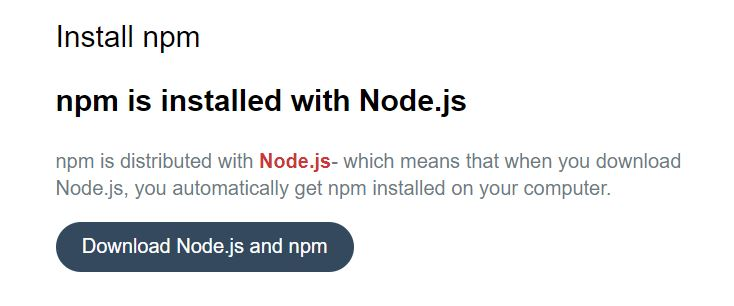
\includegraphics[scale=0.75]{Img/node}}
	\caption{Pagina di download di npm}\label{}
\end{figure}
\subsection{Installazione plug-in}
Il plug-in completo è disponibile al link \\[0.2cm]
\hspace*{10mm}\url{https://github.com/NicoloTartaggia/7DOS-plugin}\\[0.2cm]scaricabile attraverso il bottone "Clone or download" e, in seguito, "Download ZIP", oppure attraverso comando \\[0.2cm]
\hspace*{10mm}\begin{ttfamily}git clone https://github.com/NicoloTartaggia/7DOS-plugin/\end{ttfamily}\\[0.2cm]Una volta scaricato ed estratto dall'archivio compresso, spostare il contenuto all'interno del percorso specifico: 
\begin{itemize}
	\item{\begin{ttfamily}grafana-5.4.3/data/plugins\end{ttfamily}} in Windows; \item{\begin{ttfamily}var/lib/grafana/plugins\end{ttfamily} in Linux.}
\end{itemize}
Dopodiché, da terminale spostarsi all'interno della cartella del plug-in e eseguire il comando \\[0.2cm]
\hspace*{10mm}\begin{ttfamily}npm install\end{ttfamily}\\[0.2cm] per installare tutti i moduli node necessari al funzionamento del plug-in. Terminata l'installazione, procedere con il comando \\[0.2cm]
\hspace*{10mm}\begin{ttfamily}npm run build\end{ttfamily}\\[0.2cm] per eseguire il processo di build. 
Infine, riavviare il server di grafana. In Windows riaprire l'eseguibile \\[0.2cm]
\hspace*{10mm}\begin{ttfamily}grafana-server.exe\end{ttfamily}\\[0.2cm] in Linux eseguire il comando \\[0.2cm]
\hspace*{10mm}\begin{ttfamily}sudo service grafana-server restart\end{ttfamily}

\subsection{Installazione e configurazione InfluxDB}
Grafana utilizza diverse \gl{datasource} per prelevare i dati da elaborare e monitorare. In particolare, il prodotto sviluppato si appoggia ad \gl{InfluxDB}.
Di conseguenza, sono necessari due passaggi:
\begin{itemize}
	\item{Installare InfluxDB su Grafana:  dirigersi alla sezione "Configuration" dal side-menu a sinistra e selezionare la voce "Data sources". Successivamente, aggiungere una datasource tramite il bottone "Add data source" e selezionare InfluxDB. Una volta installato, impostare InfluxDB come datasource di default spuntando il relativo checkbox nelle impostazioni;}
	\item{Scaricare InfluxDB al link \\[0.2cm]
		\hspace*{10mm}\url{https://portal.influxdata.com/downloads/}.\\[0.2cm] La versione di riferimento utilizzata durante lo sviluppo è la 1.7. Una volta scaricato, avviare il server. In Windows, eseguire \\[0.2cm]
		\hspace*{10mm}\begin{ttfamily}influxd.exe\end{ttfamily}\\[0.2cm] mentre in Linux eseguire il comando \begin{ttfamily}sudo service influxdb start\end{ttfamily}.\\}
	L'istanza sarà interrogabile all'indirizzo \url{localhost:8086}.
\end{itemize}

\pagebreak